\chapter{Max cut}

We have been talking about minimal cuts the whole time. Now we will consider somewhat opposite problem. That is for given graph $G = (V,E)$ we want to find $S \subseteq V$ such that $E(S, V \setminus S)$ is maximized.

For this problem we may introduce a \textbf{randomized algorithm} which is simple. For every vertex choose if it is in $S$ or in $V \setminus S$ with probability $1/2$. Then $\E [|E(S, V \setminus S)|] = \frac{|E|}{2} \geq \frac{OPT}{2}$ because the probability of edge being in the cut is exactly one half, since there are four options where $u$ and $v$ may land, but in two scenarios they are in the same part and in the rest they are on the opposite sites.

Now we would like to talk about $0,878\dots$-approximation. Firstly we will label our vertices. WLOG: $V = \{1, 2, \dots, n\}$. Set $\forall i \in V: y_{i}^2 =1$. Now think about an edge $ij$. How can we express with this representation of the graph that $ij$ is in the cut? Think about

$$
y_{i} \cdot y_{j} = \left\{
\begin{array}{r l}
	1 & \text{on the same side} \\
	-1 & \text{on different sides}
\end{array}
\right.
$$

and from this we would make

$$
\frac{1 - y_{i}\cdot y_{j}}{2} = \left\{
\begin{array}{r l}
	0 & \text{on the same side} \\
	1 & \text{on different sides}
\end{array}
\right..
$$

So with this we can introduce a maximalization problem:

$$
\max \frac{1}{2} \sum_{\{i,j\} \in E} (1 - y_i y_j)
$$

Altogether we can define a \textbf{quadratic formulation} for max-cut problem. Every part was already mentioned, but just to gather it on one place.

$$
\begin{aligned}
	\forall i \in V: y_{i}^2 = 1 \\
	\max \frac{1}{2} \sum_{\{i,j\} \in E} (1 - y_i y_j) \\
	y_{i} \in \R
\end{aligned}
$$

We may see that this program is not very good for solving. This means we will relax it to a \textbf{vector program} and we will denote it as VP for future usage.

$$
\begin{aligned}
	\max \frac{1}{2} \sum_{\{i,j\} \in E} (1 - y_i^T y_j) \\
	y_i^T y_i = 1 \\ 
	\forall i : y_{i} \in \R
\end{aligned}
$$

The intuition behind it is that we start with 1 dimensional ball (which are line segments $[-1,1]$) and then we will continue to higher dimensions. In the VP we use vectors instead of usual numbers. We will continue with changing the program. Now it will be to semi-positive programming or SPD for short. This formulation is as follows.

$$
\begin{aligned}
	\max \frac{1}{2} \sum_{\{i,j\} \in E} (1 - Y_{ij}) \\
	\forall i : Y_{ii} = 1 \\
	Y \text{ is positive semi-definite}
\end{aligned}
$$

When it is written in this form it can be solved in polynomial time. Just for a reminder we introduce a definition of PSD.

\begin{defn}
	We say that a symmetric matrix $A \in \R^{n \times n}$ is positive semi-definite if $\forall x : x^T A x \geq 0$.
\end{defn}

\begin{observ}
	$A$ is positive semi-definite $\Leftrightarrow \exists$ matrix $U \in \R^{n \times n}$ s.t. $A = U^T U$. 
\end{observ}

\begin{observ}
	VP = PSD
\end{observ}

\begin{proof}
	This is from the above observation because we can put the semi-positive matrix $Y$ to a multiplication of two matrices which will look like this:
	
	$$
	\begin{pmatrix}
		\dots & y_1 & \dots \\
		& \vdots & \\
		\dots & y_n & \dots \\
	\end{pmatrix}
	\begin{pmatrix}
		\vdots &  & \vdots \\
		y_1 & \dots & y_n\\
		\vdots &  & \vdots \\
	\end{pmatrix}
	$$
\end{proof}

\begin{algorithm}
	\caption{Algorithm for max cut}
	\begin{algorithmic}[1]
		\Require{Graph $G$}
		\Ensure{$S$ max cut of $G$.}
		\State Solve SDP.
		\State Interpret it as a solution of the VP $\to v_{1}, \dots, v_{n} \in \R^n$.
		\State Sample uniformly at random $r \in \{x \in \R^n : x^2 = 1\}$
		\State \Return $S = \{i \in V : v_{i}^T r \geq 0\}$.
	\end{algorithmic}
\end{algorithm}

We know that both $v_{i}$ and $r$ are unit vectors. So $\cos \alpha = v_{i}^T \cdot r$. Where the $\cos$ function can be seen on a picture \ref{cos} to visualize how it looks.

\begin{figure}[!ht]\centering
	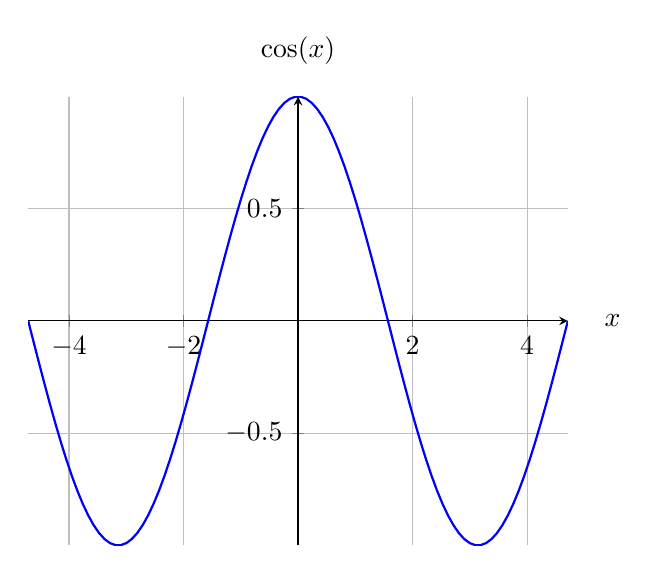
\begin{tikzpicture}
		\begin{axis}[
			xlabel=$x$,
			ylabel=$\cos(x)$,
			domain=-3/2*pi:3/2*pi,
			samples=100,
			axis lines=middle,
			grid=both,
			every axis y label/.style={at={(ticklabel* cs:1.05)}, anchor=south},
			every axis x label/.style={at={(ticklabel* cs:1.05)}, anchor=west},
			]
			\addplot[blue, thick] {cos(deg(x))};
		\end{axis}
	\end{tikzpicture}
	\caption{Cosine function.}
	\label{cos}
\end{figure}

Now we will take a step back and try to achieve the mysterious number for the approximation ratio. Let $\theta_{ij}$ be the angle between $v_{i}$ and $v_{j}$. Then for $\{i,j\} \in E$, its contribution to the objective (in VP) is $\frac{1 - \cos \theta_{ij}}{2}$.

\begin{lemma}[no proof]
	For each $x \in \langle 0, \pi \rangle$ and $\alpha = 0,87856$ it holds that
	
	$$
	\frac{x}{\pi} \geq \alpha \frac{1 - \cos x}{2}
	$$
\end{lemma}

The meaning of it is shown on the picture \ref{meaning}.

\begin{figure}[!ht]\centering
	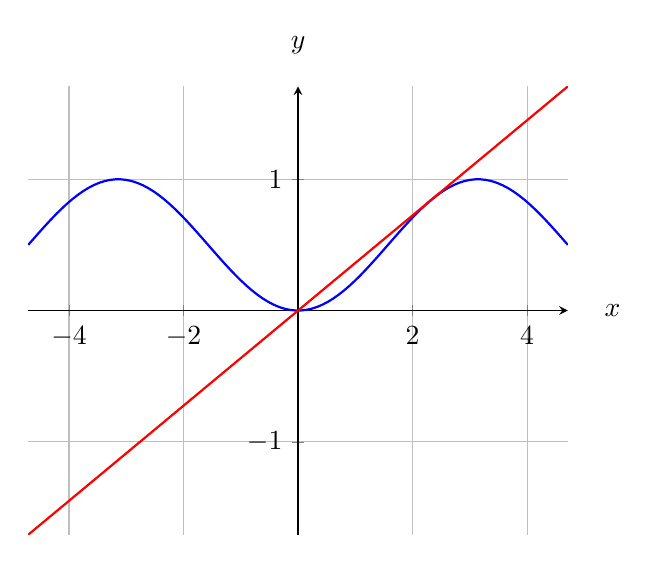
\begin{tikzpicture}
		\begin{axis}[
			xlabel=$x$,
			ylabel=$y$,
			domain=-3/2*pi:3/2*pi,
			samples=100,
			axis lines=middle,
			grid=both,
			every axis y label/.style={at={(ticklabel* cs:1.05)}, anchor=south},
			every axis x label/.style={at={(ticklabel* cs:1.05)}, anchor=west},
			legend pos=outer north east,
			]
			\addplot[blue, thick, label=($(1 - \cos(x)) /2$)] {(1 - cos(deg(x))) / 2};
			\addplot[red, thick, label=($x/(\pi \cdot \alpha)$)] {x / (0.87856 * pi)};
			\legend{}
		\end{axis}
	\end{tikzpicture}
	\caption{The \textcolor{red}{red} function is for $x/(\pi \cdot \alpha)$ and \textcolor{blue}{blue} for $(1 - \cos(x)) /2$.}
	\label{meaning}
\end{figure}

\begin{lemma}
	For $\{i,j\} \in E$ $\Pr [i \text{ and } j \text{ are separated}] = \frac{\theta_{ij}}{\pi}$.
\end{lemma}

\begin{proof}
	Consider the projection of $r$ to the plane defined by $v_i$, $v_j$. Let $W$ be the objective value of our solution:
	
	$$
	\begin{aligned}
		\E [W] & =    & \sum_{\{i,j\} \in E} \frac{\theta_{ij}}{\pi} & \quad \text{(by linearity of expectation)} \\
		       & \geq & \alpha \sum_{\{i,j\} \in E} \frac{1 - \cos (\theta_{ij})}{2} & \quad \text{(by the first lemma)} \\
		       & =    & \alpha \sum_{\{i,j\} \in E} \frac{1 - v_{i}^T v_{j}}{2} & \quad \textbf{(this is our objective functions of VP)} \\
		       & \geq & \alpha \cdot OPT & \quad \text{(because VP is a relaxation)}
	\end{aligned}
	$$
\end{proof}